\documentclass{cys}

\usepackage[utf8]{inputenc}

%\usepackage[english]{babel}
%\usepackage[spanish,mexico,es-tabla]{babel}
\usepackage[russian,english]{babel}  % If you use other languages, use Babel package.


\usepackage{graphicx}
\usepackage{subcaption}
\usepackage{multirow}

\usepackage{epstopdf} % Avoid using plain Latex, use PDFLATEX

\addto\captionsenglish{%
  \renewcommand{\figurename}{Fig.}%
  \renewcommand{\abstractname}{Abstract.} 
%  \renewcommand{\keywordsname}{Keywords: } 
}

\addto\captionsspanish{%
  \renewcommand{\figurename}{Fig.}%
  \renewcommand{\abstractname}{Resumen.} 
%  \renewcommand{\keywordsname}{Palabras clave: } 
}


\title{Self-driving	Through a Deep Recurrent Convolutional Neural Model}

\author{Antonio Luna-Álvarez, Dante Mújica-Vargas}

\affil{ 
Tecnológico Nacional de México CENIDET, Departament of Computer Sciences , Cuernavaca, \authorcr   % Do not us full postal address!
México             
\authorcr  \authorcr
jesus.luna18ce@cenidet.edu.mx, dantemv@cenidet.edu.mx
\authorcr  \authorcr
}


\begin{document}

\maketitle

\renewcommand{\tablename}{Table}

\begin{abstract}
This paper presents...
\end{abstract}

\begin{keywords} 
Deep Learning, Convolutional Model, Recurrent Model, Time-distributed, Self-driving, Autonomy.
\end{keywords} 

%%%%%%%%%%%%%%%%

\section{Introduction}
\label{sec:introduction}
% PARRAFO 1: PROBLEMA A TRATAR
Autonomous vehicles are robotic systems that must have the ability to navigate through the environment for which they were designed, independently and avoiding obstacles or situations that compromise the safety of the vehicle and its passengers, this task is named self-driving. The main component of a self-driving car is the decision module, which can be controlled by a classification model that will mainly predict the steering angle and vehicle speed.


% PARRAFO 2 Y 3: ESTADO DEL ARTE
Good results on self-driving have been documented using deep learning. Among the best are the research department of Nvidia, that proposes a convolutional deep model called Pilotnet \cite{bojarski2016end}\cite{bojarski2017explaining} to provide autonomous driving in simulation and a physical system. Other authors have used this model to perform experiments on open source simulators \cite {alexeev2018end}.

There are also other deep neural models proposed with different architectures and paradigms, a reference is \cite{tian2018deeptest}, which evaluates these models to detect prediction errors and possible collisions in static images. Using images of roads, compares two convolutional models like Pilotnet and a recurrent LSTM model getting better results with the last one.


% PARRAFO 4: ANALISIS DEL EDO ART (OPORTUNIDADES)
Although satisfactory results have been reported, a deficiency has been detected in these. Particularly the driving task is an activity that depends on the actions taken in previous moments to take a new decision that controls the course of the vehicle. For example, a vehicle that just made a change of course. A reactive model such as those mentioned above, only receives the information of the current scene as shown in Fig. \ref{subfig:reactive}, consequently it will provide a response that is valid for straight roads. However, a time-based model obtains information from previous scenarios such as Fig. \ref{subfig:recurrent}, thus allowing corrections and a response similar to that made by a human driver.

\begin{figure}[h]
	\centering
	\begin{subfigure}{0.22\textwidth} 
		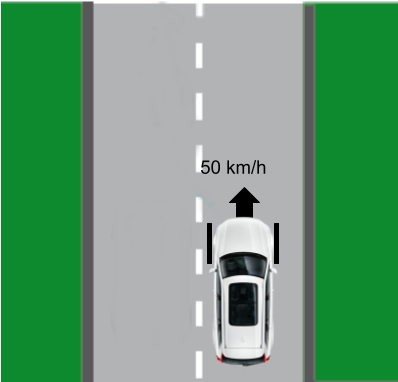
\includegraphics[width=\textwidth]{img/reactive}
		\subcaption{Scene that sees a reactive model} 
		\label{subfig:reactive}
	\end{subfigure}
	\begin{subfigure}{0.211\textwidth} 
		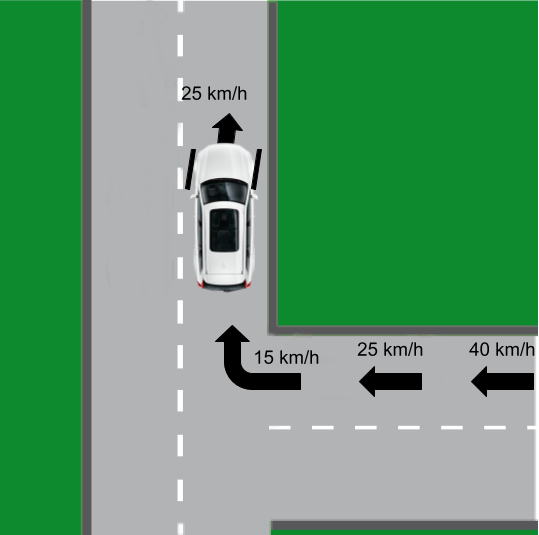
\includegraphics[width=\textwidth]{img/recurrent}
		\subcaption{Scene that sees a model based on time} 
		\label{subfig:recurrent}
	\end{subfigure}
	\caption{Difference between reactive and time-based models} 
	\label{fig:comparsion}
\end{figure}


% PARRAFO 5: VENDER PROPUESTA
In order to offer a solution to this deficiency, it is proposed to use a recurrent convolutional model that satisfies the need to make decitions based on time. Since recurrent networks have been used to identify relationships between succession of data \cite{bianchi2017recurrent}, they are used to classify actions from a sequence of images processed by convolutional layers of the model as in other works. Based on the Chauffeur model \cite{tian2018deeptest}, is adapted to receive sequences of images, thus creating time-distributed convolutional layers, and recurrent layers are used to make the clasifications based on the obtained information.

% PARRAFO 6: CONTENIDO DEL DOCUMENTO
In the next section is presented the theoretical concepts necessary to understand the functioning of recurrent and convolutional neuronal models. Also in the section \ref{sec:systemDescription} the implementation made with the neural models and the Udacity simulator is shown. In the section \ref{sec:experiments} there is evidence of the results obtained, to finally give the final conclusions and acknowledgments in the last section.

\section{Background}
\label{sec:Background}

% PARRAFOS 7 - 12: SINTESIS DE CONCEPTOS TEORICOS
\subsection{Recurrent Neural Network}
Recurrent neural networks have been used in natural language processing to find relationships between word sequences and their dependence in the long and short term \cite{bianchi2017recurrent}. In the same way these networks are used to find relationships between the scenes shown.

There are three types of essential tasks that can be performed with this type of network \cite{bonet2007redes}:

\begin{enumerate}
	\item Sequence recognition: A particular output pattern occurs when an input sequence is specified.
	
	\item Sequence playback: The network must be able to generate the rest of a sequence when you see part of it.
	
	\item Temporal association: In this case a particular output sequence must be produced in response to a specific input sequence.\\
\end{enumerate}

The Long Long-term Memory (LSTM) architecture was originally proposed by Hochreiter and Schmidhuber in 1997 \cite{hochreiter1997long}, and is widely used today due to its superior performance in accurate modeling of short and long term dependencies.

An LSTM neuron is composed of 5 different non-linear components, which interact with each other in a particular way. In this paradigm, 4 components are called gates, they protect and control the information in the cell, which stores the memory of the neuron. The gates are implemented by a sigmoid function $\sigma(\cdot)$ and Hadamard product $\odot$. To control the behavior of each gate, one trains with a set of parameters and by calculating the gradient descending. The 5 gates of an LSTM cell are expressed as:

\begin{equation}
Forget: \sigma_f[t] = \sigma(\textbf{W}_f x[t]+\textbf{R}_f y[t-1]+b_f) 
\end{equation}    
\begin{equation}
Candidate: \tilde{\textbf{h}}_f[t] = g_1(\textbf{W}_h x[t]+\textbf{R}_h y[t-1]+b_h)
\end{equation}
\begin{equation}
Update: \sigma_u[t] = \sigma(\textbf{W}_u x[t]+\textbf{R}_u y[t-1]+b_u)
\end{equation}
\begin{equation}
Cell: \textbf{h}[t] = \sigma_u[t] \odot \tilde{\textbf{h}}[t]+\sigma_f[t]\odot \textbf{h}[h-1]
\end{equation}
\begin{equation}
Output\ g: \sigma_o[t] = \sigma(\textbf{W}_o\textbf{x}[t]+\textbf{R}_o y[t-1]+\textbf{b}_o)
\end{equation}
The final classification is made by:
\begin{equation}
Output: \textbf{y}[t] = \sigma_o[t]\odot g_2(\textbf{h}[t])
\end{equation}

Where $x[t]$ is the input vector at time $t$. $W_f$, $W_h$, $W_u$ and $W_o$ are rectangular weight matrices that are applied to the input of the LSTM cell. $R_f$, $R_h$, $R_u$ and $R_o$ are square matrices that define the weights of the recurrent connections, while $b_f$, $b_h$, $b_u$ and $b_o$ are vectors of bias. The function $\sigma(\cdot)$ is sigmoid, while $g_1(\cdot)$ and $g_2(\cdot)$ are point nonlinear activation functions generally implemented as hyperbolic tangents that reduce the values in $[-1, 1]$. Finally, $\odot$ represents the inner product \cite{bianchi2017recurrent}. 


\subsection{Convolutional Neural Network}
This type of neural network has great advantages of automation in the task of extracting image information. In this paradigm, no known image processing filter is applied, but through the training of the neural network, it learns the image processing filters. The CNN is based on the convolution of signals in two dimensions and the detection of filter-based characteristics (called kernel) that they learn through training. To extract the characteristics, the kernel performs the 2D convolution operation, expressed in \ref{eq:convolution}, to the input image. 

\begin{equation}
y(n_1, n_2) = \sum_{k_2=0}^{N-1} \sum_{k_1=0}^{M-1} x(k_1, k_2)\ h(n_1 - k_1, n_2 - k_2)
%0 \leq n_1 \leq N-1,\ 0 \leq n_2 \leq M - 1
\label{eq:convolution}
\end{equation}

Where $N$ and $M$ are the dimensions of the image, $n_1$ and $n_2$ represent the column and row indices of the pixel being processed, $k_1$ and $k_2$ the kernel indexes. These indices must meet the condition: $0 \leq n_1 \leq N-1,\ 0 \leq n_2 \leq M - 1$ \cite{pattanayak2017pro}.


To train the convolutional layers, the backpropagation through the convolutional layer technique is used. This is very similar to backpropagation for a multilayer perceptron network, the only difference being that the weight connections are scattered, since the different input areas share the same weights to create a map of output characteristics. In general, the map of characteristics is obtained through the function expressed in \ref{eq:error}. Where $w$ represents the weights of the kernel and a first map of characteristics obtained.

\begin{equation}
S_{ij} = \sum_{n=1}^{2} \sum_{m=1}^{2} w_{(3-m)(3-n)} \cdot a_{(i-1+m)(j-1+m)}
\label{eq:error}
\end{equation}

For convolutional layers, the assigned activation function is the Rectified Linear Unit Function (ReLU) which is expressed in \ref{eq:relu} where $x$ represents the input value. This function allows normalizing the data by not admitting negative values and thus avoid noise that may contain the input image.

\begin{equation}
ReLU = ln(1+e^x)
\label{eq:relu}
\end{equation}

On the other hand, the kernel weights are adjusted by calculating the descending gradient which is expressed in \ref{eq:gradient}. Where $L$ represents the error function.
\begin{equation}
\frac{\partial L}{\partial w_{ij}} = \sum_{i=1}^{2} \sum_{j=1}^{2} \frac{\partial L}{S_{ij}} \frac{\partial S_{ij}}{\partial w_{ij}}
\label{eq:gradient}
\end{equation}



\section{System Description}
\label{sec:systemDescription}
% PARRAFO 13 - 20: DESCRIPCIÓN MATEMÁTICA
% PSUDOCODIGOS, DIAGRAMAS, EXP MAT, ESQUEMAS


\section{Experiments \& Results}
\label{sec:experiments}
% PARRAFO 21 - 23: PERTINENCIA DE LOS EXPERIMENTOS


% PARRAFO 24 - 28: MENCIONAR METODOS CON LOS QUE SE COMPARA

To compare the results,the NVIDIA Pilotnet model \cite{bojarski2016end}\cite{bojarski2017explaining} was replicated  shown in Fig. \ref{fig:pilotnet}. This model is the greatest reference in the self-driving domain and unlike the Chauffeur model (Fig. \ref{fig:chauffeur}), it doesn't have convolutional layers of distributed time and its classification is based only on multilayer perceptron.

\begin{figure}[h]
	\centerline{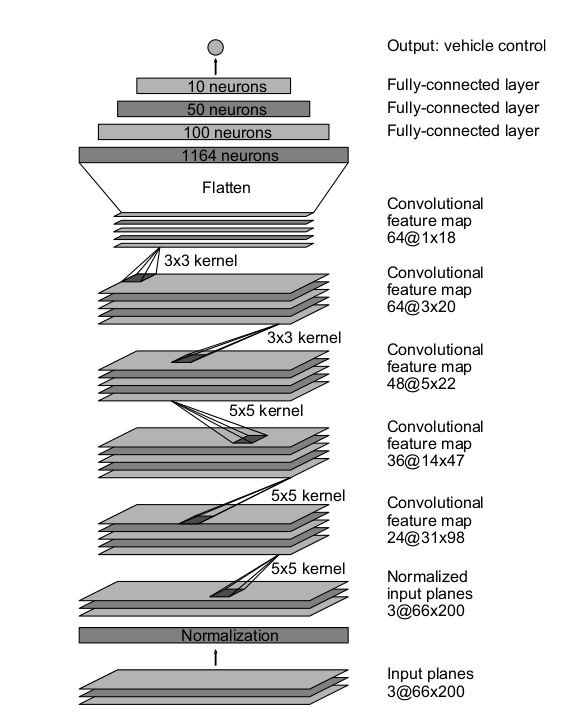
\includegraphics[scale=0.33]{img/pilotnet}}
	\caption{Pilotnet model \cite{bojarski2016end}.}
	\label{fig:pilotnet}
\end{figure}

The tuning of parameters is the same for both models:
\begin{itemize}
	\item Epochs: 10.
	\item Iterations: 10,000.
	\item Lot: 40 patterns.
	\item Learning rate: $1.0^{-5}$.
	\item Training set: 80\%.
	\item Validation set: 20\%.
\end{itemize}

To compare the results with the Chauffeur model with different steps, it was trained with 3 and 5 steps using the same parameter configuration.


% PARRAFO 29 - 30: HARDWARE/SOFTWARE UTILIZADO

The training of a deep neuronal model requires great computational processing capacity, due to this the implementation was carried out with the support of special frameworks for the processing parallelization. The implementation was carried out with the help of the following software:

\begin{itemize}
	\item OS: Xubuntu 14.04 Trusty Tahr.
	\item Udacity Simulator precompiled.
	\item Python 3.4.
	\item Tensorflow 1.1.0 (gpu support).
	\item Keras 2.1.2.
	\item CUDA Driver 8.0.
	\item cuDNN Driver 5.1.
\end{itemize}

In turn, this software requires high performance hardware, so a computer was used with the following characteristics:

\begin{itemize}
	\item CPU Intel Core 17-7700 3.60 GHz, 4 cores 8 threads.
	\item 12 GB RAM.
	\item 1 TB HDD.
	\item 120 GB SSD.
	\item GPU GeForce GTX TITAN X 3072 CUDA cores, 12 GB, 1000 MHz.
\end{itemize}


% SUBSECCIÓN: 
% MÉTRICAS, BD, EXPERIMENTOS
\subsection{Metrics}

Remembering that the problem have 87 classes, a difference of 0.01 in the prediction represents an absolute error in the metrics that are usually used for the evaluation of neural networks, such as precision, accuracy, etc. However, in the tests, a minimal error doesn't have such a drastic effect on driving, that is why this type of evaluation doesn't turn out to be ideal.

On the other hand, the metrics dedicated to measure the error in the prediction adapt much better to the problem and show the performance of these networks, since they calculate the difference between the expected and the obtained. A small angle of difference doesn't present as much error, that is why these are the ones that were contemplated to evaluate the training of the networks. The metrics used are: Mean Squared Error \ref{eq:mse} and Mean Absolute Error \ref{eq:mae}.

\begin{equation}
	MSE = \frac{1}{n} \sum_{i=1}^{n} = (\hat{Y_i} - Y_i)^2
	\label{eq:mse}
\end{equation}
\begin{equation}
	MAE = \frac{1}{n} \sum_{i=1}^{n} = |\hat{Y_i} - Y_i|^2
	\label{eq:mae}
\end{equation}



In the study of the state of the art, few metrics related to the evaluation of autonomy were found. In \cite{bojarski2016end}, the metric shown in \ref{eq:nvidia} is proposed, which is the most referenced in the literature.

\begin{equation}
autonomy = (1 - \frac{interventions \cdot 6}{elapsed\ time}) \cdot 100
\label{eq:nvidia}
\end{equation}

The metric is based mainly on the corrections made by the driver to avoid collision of the vehicle. This number of interventions is multiplied by a constant of 6 seconds, which represents the average time an average driver takes to correct the course of the vehicle, according to a study carried out by them.

Throughout the tests carried out in this work it was observed thatn't necessarily an intervention is usually 6 seconds in the simulation, even though it's in real time. Due to these variations, the metric proposed in the literature turns out to be less reliable, therefore it's proposed to measure the autonomy based on the intervention time of the driver to correct the address using the expression \ref{eq:proporsed}. This proposed metric evaluates the autonomy similarly to the previous one, with the difference that it takes an absolute time of interventions.

\begin{equation}
autonomy = (1 - \frac{total\ intervention\ time}{elapsed\ time})\cdot 100
\label{eq:proporsed}
\end{equation}

As a third autonomy metric, it's proposed to perform the test without the driver's intervention to measure the percentage of the route that completes the vehicle on the runway until the first collision using the expression \ref{eq:completed road}. In this way there's a reference on what each model He has learned from the road.

\begin{equation}
completed\ road = \frac{s \cdot t}{d} \cdot 100
\label{eq:completed road}
\end{equation}

Where $s$ is the average speed of the vehicle, $t$ represents the driving time until the first collision or completing the route and $d$ is the total distance of the test track.

 
Although there are metrics to evaluate the training quality of the neuronal model and the autonomy of the vehicle, during the experimentation it was observed that, although without colliding, the vehicle has to approach the ends of the road and change lanes in the form of zigzag. Because there is no collision, autonomy metrics do not penalize to the driving. Therefore, a metric based on the standard deviation \ref{eq:std} \cite{spiegel1991estadistica} is proposed.

\begin{equation}
s = \sqrt{\frac{\displaystyle\sum_{j=1}^{N} (x_j - \bar{x})^2}{N}}
\label{eq:std}
\end{equation}


This metric depends on a reference line previously made by a person. The standard deviation of the steering angle of the steering wheel made during driving is calculated, in the same way it is calculated for all the predictions of the neural model. Finally, the absolute difference of these deviations is calculated, obtaining an error in the conduction behavior in the function \ref{eq:abs}.

\begin{equation}
	conduct = |s-s'|
	\label{eq:abs}
\end{equation}


% GRAFICAS, TABLAS, VISUALIZACIÓN
\subsection{Results}

\begin{table*}[H]
	\caption{Metrics of autonomy obtained.}
	\begin{center}
		\begin{tabular}{|c|c|c|c|c|}
			\hline
			\multirow{3}{*}{\textbf{Model}} & \multicolumn{4}{|c|}{\textbf{Metrics}} \\\cline{2-5} 
			& \multicolumn{2}{|c|}{NVIDIA} & \multicolumn{2}{|c|}{Proporsal} \\\cline{2-5} 
			& Road 1 & Road 2 & Road 1 & Road 2 \\\hline \hline
			
			Pilotnet (shortest db) & 44.55\% & 83.11\% & 82.09\% & 96.35\% \\\hline
			Pilotnet (largest db) & \textbf{100\%} & 77.57\% & \textbf{100\%} & 90.05\% \\\hline
			Chauffeur 3 steps (shortest db) & 76.88\% & 85.96\% & 90.26\% & 92.48\% \\\hline
			Chauffeur 3 steps (largest db) & \textbf{100\%} & \textbf{100\%}   & \textbf{100\%} & \textbf{100\%} \\\hline
			Chauffeur 5 steps (shortest db)& 88.89\% & 88.78\% & 95.43\% & 96.23\% \\\hline
			Chauffeur 5 steps  (largest db)& \textbf{100\%} & \textbf{100\%} & \textbf{100\%} & \textbf{100\%} \\\hline
		\end{tabular}
		\label{table:autonomy}
	\end{center}
\end{table*}

\begin{table*}[H]
	\caption{Metrics of road completed obtained.}
	\begin{center}
		\begin{tabular}{|c|c|c|}
			\hline
			\multirow{2}{*}{\textbf{Model}} & \multicolumn{2}{|c|}{\textbf{Road completed}} \\\cline{2-3} 
			& Road 1 & Road 2 \\\hline \hline
			
			Pilotnet (shortest db) & 9.47\% & 7.52\% \\\hline
			Pilotnet (largest db) & \textbf{100\%} & 30.44\% \\\hline
			Chauffeur 3 steps (shortest db) & 33.61\% & 18.07\% \\\hline
			Chauffeur 3 steps (largest db) & \textbf{100\%} & \textbf{100\%} \\\hline
			Chauffeur 5 steps (shortest db) & 34.37\% & 16.93\% \\\hline
			Chauffeur 5 steps (largest db) & \textbf{100\%} & \textbf{100\%} \\\hline
		\end{tabular}
		\label{table:read}
	\end{center}
\end{table*}


\begin{figure*}[h]
	\centering
	\begin{subfigure}{0.32\textwidth} 
		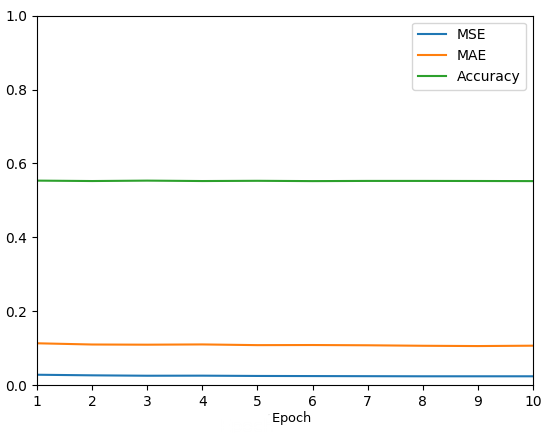
\includegraphics[width=\textwidth]{img/pilotnet1}
		\subcaption{Pilotnet, largest database.} 
		\label{subfig:1}
	\end{subfigure}
	\begin{subfigure}{0.32\textwidth} 
		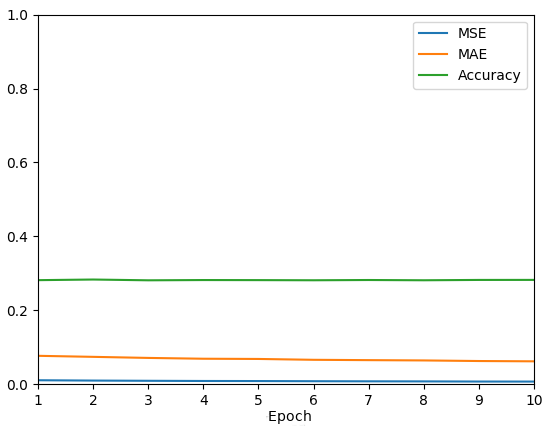
\includegraphics[width=\textwidth]{img/pilotnet2}
		\subcaption{Pilotnet, shorter database.} 
		\label{subfig:2}
	\end{subfigure}
	\begin{subfigure}{0.32\textwidth} 
		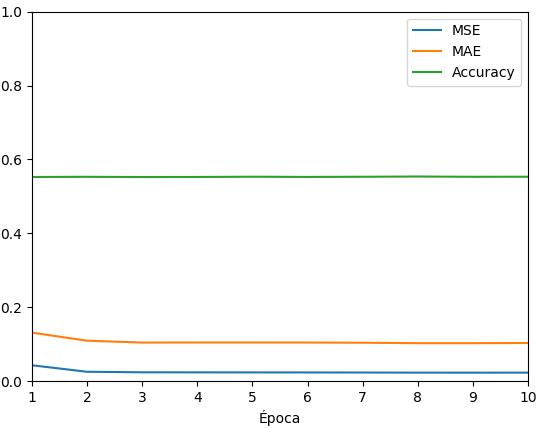
\includegraphics[width=\textwidth]{img/chauffeur3}
		\subcaption{Chauffeur 3 steps, largest database.} 
		\label{subfig:3}
	\end{subfigure}
	\begin{subfigure}{0.32\textwidth} 
		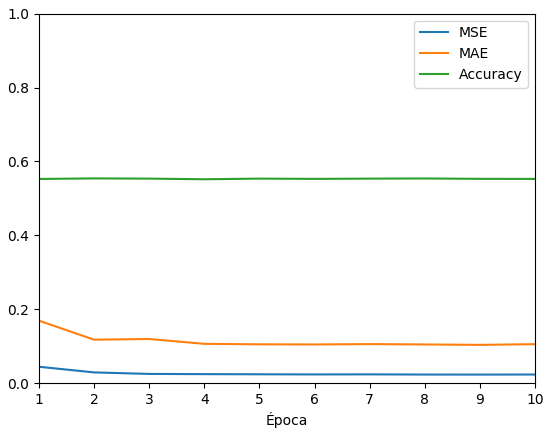
\includegraphics[width=\textwidth]{img/chauffeur5}
		\subcaption{Chauffeur 5 steps, largest database.} 
		\label{subfig:4}
	\end{subfigure}
	\begin{subfigure}{0.32\textwidth} 
		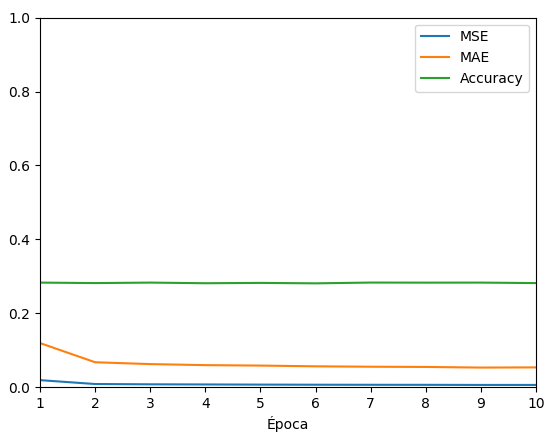
\includegraphics[width=\textwidth]{img/chauffeur3m}
		\subcaption{Chauffeur 3 steps, shorter database.} 
		\label{subfig:5}
	\end{subfigure}
	\begin{subfigure}{0.32\textwidth} 
		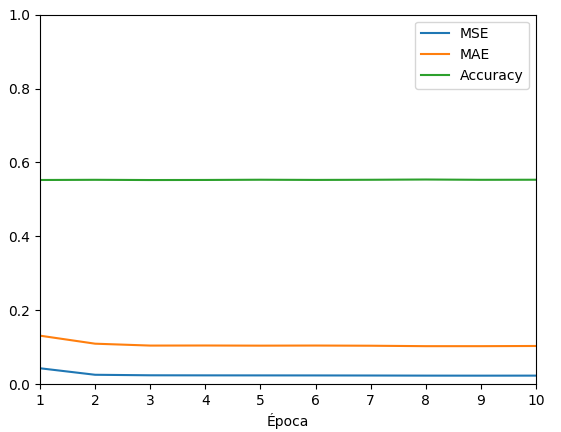
\includegraphics[width=\textwidth]{img/chauffeur5m}
		\subcaption{Chauffeur 5 steps, shorter database.} 
		\label{subfig:6}
	\end{subfigure}
	\caption{Training metrics obtained.} 
	\label{fig:pilottest}
\end{figure*}


% SUBSECCIÓN:
% DISCUSIÓN DE RESULTADOS
\subsection{Result Discussion}

\section{Conclusion and Future Work}
\label{sec:conclusionAndFutureWork}

% CONCLUSION Y TRABAJO FUTURO

Conclusions here.

\section*{Acknowledgements} 
We would like to thank.. 
This work is funded by...


%\begin{table}[ht]
%	\renewcommand{\arraystretch}{1.3}
%	\centering
%	\caption{Tables, no capital letters, no point at the end}
%	\begin{tabular}{lrrrr}
%		\hline
%		Classes & Articles \\
%		\hline
%		one \emph{and} two& 61 & 115,729 \\
%		three & 169 & 869,607 \\
%		four & 209 & 2,402,704 \\
%		five & 206 & 2,561,115 \\		
%		\hline
%	\end{tabular}
%	\label{table:Table1}
%\end{table}

% OBLIGATORY: use BIBTEX formatting!
\small{
\bibliographystyle{cys}
\bibliography{biblio}
}
\normalsize


\begin{biography}[]{} % Leave this section empty
\end{biography}

{\vskip 12pt}
\noindent
\footnotesize {\textit{Article received on 06/12/2016; accepted on 16/01/2017.\\
Corresponding author is XXXXX.}

\end{document}
